% ================================================
% =              STATE OF THE ART                =
% ================================================ 

Actualmente, la industria de la automoción está impulsando el desarrollo de los \aclink{ADS} con la promesa de reducir los accidentes en carretera y minimizar los costes tanto humanos como económicos que estos suponen \cite{survey_AutomatedDriving1}. Sin embargo, a pesar de que la conducción automatizada haya incrementado recientemente la atención de la industria por el auge del DeepLearning y la visión por ordenador, lo cierto es que lleva presente más de 20 años.

Algunas de las primeras competiciones de conducción automatizada, como los DARPA Challenges en 2003 y 2005 o el Grand DARPA Urban challenge de 2007, impulsaron enormemente el desarrollo de los \aclink{ADS}, atrayendo la atención tanto de empresas tecnológicas como del sector automotriz \cite{survey_AutomatedDriving2}. Este avance ha sido acompañado por la definición de buenas prácticas y procesos de estandarización para garantizar la seguridad y fiabilidad de los \aclink{ADS}. En este contexto, la \aclink{SAE} ha establecido una escala progresiva de automatización, desde el nivel 0 (sin automatización) hasta el nivel 5 (automatización total), definiendo el grado de intervención del conductor en cada etapa \cite{AD_Technical_Standards}. 

Hoy en día, la mayoría de los vehículos incorporan sistemas avanzados de asistencia a la conducción \aclink{ADAS}, que operan en los niveles \aclink{SAE} 2 y 3. No obstante, ya existen \aclink{ADS} de nivel 4, como los desarrollados por Waymo y Cruise para robotaxis, o los autobuses autónomos desplegados en algunas ciudades, cuyos sistemas están diseñados para gestionar el fallback de manera autónoma, sin necesidad de intervención humana \cite{fallback_strategy}.

Este desarrollo ha llevado a la creación de distintas estrategias y arquitecturas para los \aclink{ADS}. En los últimos años, ha habido grandes avances en soluciones \mbox{End-to-End}, que combinan técnicas de aprendizaje profundo y aprendizaje por refuerzo para obtener las acciones de control del vehículo partiendo diréctamente de los datos de los sensores \cite{end_to_end_driving}. Sin embargo, la mayoría de los enfoques optan por soluciones modulares más tradicionales, que dividen el problema de la conducción automatizada en \mbox{sub-tareas} específicas, integrando soluciones de campos como la robótica, visión por ordenador, deep learning y control automático.

En el contexto de las arquitecturas modulares, la adopción de buenas prácticas ha facilitado la categorización de estas \mbox{sub-tareas} en tres grupos principales \cite{machines5010006}\cite{functional_architectures}: 
\begin{itemize}
    \item Percepción, que se refiere a la capacidad del sistema autónomo para recolectar información del entorno y extraer conocimiento relevante, como la ubicación de obstáculos, señales de tráfico y la localización del vehículo.
    \item Planificación del comportamiento, que consiste en tomar decisiones para alcanzar los objetivos del vehículo, como llegar de un punto a otro evitando obstáculos y optimizando la trayectoria.
    \item Ejecución de movimientos, que se refiere a la capacidad del vehículo para ejecutar las acciones planificadas por el sistema, controlando la dirección, velocidad y maniobras necesarias.
\end{itemize}
Además, estas \mbox{sub-tareas} interactúan entre sí, con el hardware del vehículo y con sistemas de comunicación como \aclink{V2I} o \aclink{V2X} en el caso de los vehículos conectados.

\begin{figure}[H]
    \centering
    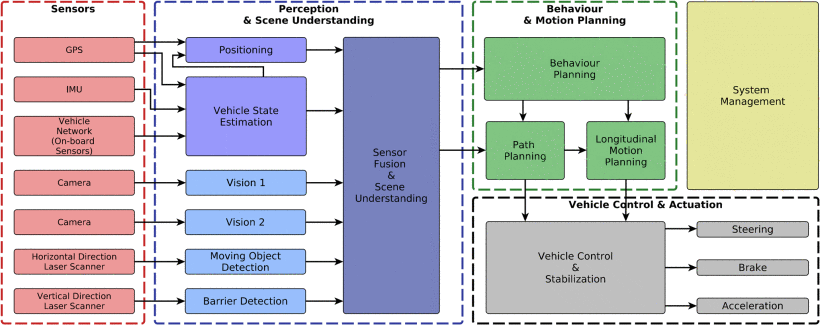
\includegraphics[width=\linewidth]{images/sota/ADS_information_flow.png}
    \label{sota_ads_information_flow}
    \caption{Arquitectura modular de un ADS. TEMPORAL!!!}
\end{figure}

En este tipo de arquitecturas, un error en una \mbox{sub-tarea} puede propagarse y afectar el desempeño de otras, comprometiendo así el funcionamiento del sistema. Esto es especialmente crítico en el módulo de percepción, ya que la calidad de la información obtenida impacta directamente en tareas posteriores como la localización, el mapeo y la planificación. Por ello, garantizar sistemas de percepción robustos es fundamental para el rendimiento y la seguridad de los \aclink{ADS}.

Dos de las tareas principales de los sistemas de percepción en los \aclink{ADS} son la detección 3D de objetos y la segmentación en \aclink{BEV}. La detección 3D de objetos es una de las tareas más relevantes y comúnmente se basa en nubes de puntos obtenidas mediante sensores LiDAR. En ausencia de LiDAR, una alternativa es la detección 3D multi-cámara, que busca predecir cajas delimitadoras 3D en un sistema de coordenadas \aclink{BEV} utilizando únicamente imágenes monoculares. Por otro lado, la segmentación en \aclink{BEV} tiene como objetivo realizar una segmentación semántica del entorno, identificando áreas transitables y delimitaciones de carril en el marco de referencia del vehículo. A diferencia de la detección de objetos, la segmentación en \aclink{BEV} permite una predicción densa de clases estáticas del entorno, lo que resulta clave para la construcción de mapas locales, estimación del comportamiento de agentes y downstream tasks como la planificación del comportamiento del \aclink{ADS}. \hl{Añadir referencias.}

% Parrafo conector que no se me ocurre nada
Este \aclink{TFM} se desarrolla en el contexto de la segmentación semántica en \aclink{BEV}\dots \hl{COMPLETAR.}


\subsection{Segmentación semántica}
\lipsum[2-4]

\subsection{Segmentación semántica en BEV}
\lipsum[1-1]


